\documentclass{article}
\usepackage[utf8]{inputenc}
\usepackage[danish]{babel}
\usepackage{graphicx}
\usepackage{url}

\title{Boblesortering}
\author{
	\begin{tabular}{l r}
		Lukas Villumsen & (s144451)\\
		Sebastian Nyholm & (s144434)\\
	\end{tabular}
}

\begin{document}
\maketitle

\section*{Resumé}
	Dette dokument omhandler boblesortering. Der beskrives algoritmen og præsenteres en kompleksitetanalyse.

\section{Introduktion}
	Boblesortering (\textit{eng. bubble sort}) er en populær \emph{\textbf{sorteringsalgoritme}} og er en af de simpleste algoritmer at forstå og implementere. Dog er den ikke en særlig effektiv sorteringalgoritme\footnote{Mere om dette i "Algoritmer og Datastrukturer 1"}; hverken for store eller små lister, og den anvendes sjældent i praksis. Boblesortering sorterer, som navnet antyder, elementerne i en list ved at \emph{boble} hvert element gennem listen til sin rette plads i listen.

\subsection{Pseudokode}
	Wikipedia~\cite{wiki} giver følgende pseudokode for boblesortering.

	\begin{verbatim}
	procedure bubbleSort(A : list of sortable items) defined as:
  	 do
     	swapped := false
     	for each i in 0 to length(A) - 2 inclusive do:
     	  if A[i] > A[i+1] then 
    	     swap(A[i], A[i+1])
    	     swapped := true
    	   end if
     	end for
   	while swapped
	end procedure

	\end{verbatim}
	En illustration af en kørsel af boblesortering fra Wikipedia kan ses på figur~\ref{figur1}

\section{Analyse af boblesortering}
	Antallet af sammenligninger, som boblesortering udfører på en tabel af længden n, er i værste fald
	\[\sum_{i=i}^{n-1}i=1+2+3+\cdots+n-1=\frac{n(n-1)}{2}\]
	I bedste fald er antallet n-1. Se tabel~\ref{tabel1}

	\begin{figure}[h]
		\centering
		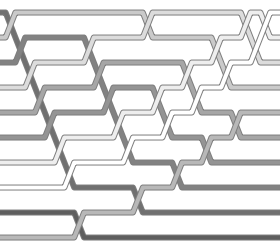
\includegraphics[scale=0.5]{Images/BubbleSort.png}
		\caption{Illustration af boblesortering.}
		\label{figur1}
	\end{figure}

	\begin{table}[h]
		\centering
		\begin{tabular}{|r|l|}
			\hline
			Værst & $n(n-1)/2$ \\
			\hline
			Bedst & $n-1$ \\
			\hline
		\end{tabular}
		\caption{Antal sammenligningner af boblesortering.}
		\label{tabel1}
	\end{table}

\section{Videre Læsning}
	For en komplet introduktion til boblesortering og relaterede sorteringsalgoritmer se Knuth~\cite{knuth}


\begin{thebibliography}{99}
		\bibitem{wiki}\textbf{http://en.wikipedia.org/wiki/Bubble\_sort}
		\bibitem{knuth}Donald Knuth, \textit{The Art of Computer Programming}, Volume 3. Addison Wesley.
\end{thebibliography}


\end{document}
